\documentclass[12pt]{beamer}

\usetheme[progressbar=frametitle]{metropolis}
\usepackage{appendixnumberbeamer}
\usepackage{csquotes}
\usepackage{booktabs}
\usepackage[scale=2]{ccicons}
\usepackage{pgfplots}
\usepgfplotslibrary{dateplot}
\usepackage{xspace}
\newcommand{\themename}{\textbf{\textsc{metropolis}}\xspace}
\usepackage{graphicx}

\title{Significant News Detection}
\subtitle{Master's Thesis}
\date{October 23, 2018}
\author{Diwas Sharma}
\institute{The University of Alabama in Huntsville}
% \titlegraphic{\hfill\includegraphics[height=1.5cm]{logo.pdf}}

\begin{document}

\maketitle

\begin{frame}{Table of contents}
  \setbeamertemplate{section in toc}[sections numbered]
  \tableofcontents[hideallsubsections]
\end{frame}

\section{Introduction}

\begin{frame}{Motivation}
    Based on a recent study \cite{matsa2018news},
    \begin{itemize}
        \item 68 percent of US adults said they at least occasionally get news on social media.
        \item However, 57 percent of those people expect the news to be largely inaccurate.
    \end{itemize}
\end{frame}

\begin{frame}{Fake news}
    \enquote{Fake news is the deliberate presentation of (typically) false or misleading claims as news, where the claims are misleading by design.} \cite{gelfert2018fake}

    Fake news viewing impacts political attitudes toward politicians \cite{balmas2014fake}, and impacts the ability of people to accept truthful news by confusing
    them with false stories \footnote{\url{https://www.nytimes.com/2016/11/28/opinion/fake-news-and-the-internet-shell-game.html?\%20r=0}}.
\end{frame}

\begin{frame}{Fake news detection}
Challenges \cite{shu2017fake},

\begin{itemize}
    \item It is difficult to classify the stories soley on content because a fake news story will try its best to appear genuine.
    \item Using auxiliary information such as knowledge base and social engagements actually leads to another problem of verifying
        the quality of the data itself.
    \item It is also impractical for human reviewers to manually categorize every single article, statement or message.
\end{itemize}

\end{frame}

\begin{frame}{Important news}
    There are articles on topics such as infotainment, personal news, beauty tips, etc. which might not have severe impact even if they were fake so they can be excluded from the
    verification step.

    For example consider following sentences,
    \begin{itemize}
        \item "I watched the Black Panther movie in the weekend. Fantastic effects!". 
        \item "There has been a shooting at the mall"
    \end{itemize}
\end{frame}

\begin{frame}{Hard/Soft news}
    \enquote{Hard news is defined as reports about politics, public administration, the economy, science, technology and related topics. Soft news is defined as reports about celebrities, human interest, sport and other entertainment-centred stories.} \cite{reinemann2012hard}

    The categorization of text into hard news and soft news is inadequate for the purpose of identifying important article from unimportant ones.
\end{frame}

\begin{frame}{Significant news}
    \enquote{A text is labeled as significant if it affects a large number of people, changes the routines of daily life, and needs verification on the information presented.}
\end{frame}

\begin{frame}{Research problems}
    \begin{enumerate}
        \item Building a new dataset for significant news detection.
        \item Studying existing fake news detection methods for detecting significant news.
        \item Selecting features from fake news detection methods and evaluating a number of classifier models for significant news detection.
    \end{enumerate}
\end{frame}

\begin{frame}{Fake news classification}
    \begin{table}[ht]
    \centering
    \begin{tabular}{ p{4cm} c r }
    \hline
    \textbf{Models} & \textbf{Classification} & \textbf{Highest Accuracy} \\
    \hline
    \textbf{Naive Bayes} & 2 class & 74\% \\
    \hline
    SVM, \textbf{SGD}, Random Forest, Bounded decision tree, and gradient boosting & 2 class & 77.2\% \\
    \hline
    Logistic regression, Bidirection LSTM, \textbf{CNN} & 6 class & 27.0\% \\
    \hline
    SVM, CNN, TCNN, \textbf{TCNN-URG} & 2 class & 89.94\% \\
    \hline
    \end{tabular}
    \caption{Fake news classification}
    \label{tbl:fake_news_classification_performance}
    \end{table}

\end{frame}

\section{Method}

\begin{frame}{Data Acquisition}
\begin{table}
    \centering
    \label{tbl:twitter_users}
    \begin{tabular}{p{3.5cm} l}
    \toprule
    Account & Link \\
    \midrule
    NYPD News & \url{https://twitter.com/nypdnews} \\
    Metropolitan Police & \url{https://twitter.com/metpoliceuk} \\
    Victoria Police & \url{https://twitter.com/VictoriaPolice} \\
    Seattle Police Dept & \url{https://twitter.com/SeattlePD} \\
    NYPD Counterterrorism & \url{https://twitter.com/NYPDCT} \\
    \bottomrule
    \end{tabular}
    \caption{Twitter accounts used for collecting data}
\end{table}
\end{frame}

\begin{frame}{Dataset labelling}
    Each article was then manually labeled as either significant news or non-significant news based on the pre-conditions
\end{frame}

\begin{frame}{Labelling sample 1}
\textbf{Text:}
\textit{Great news!! Missing 20-year-old Melissa Wilson has been located safe and well. Thank you for the shares!}\par
\textbf{Label:} Significant\par
\textbf{Reason:}
\begin{itemize}
    \item Affects a large number of people
    \item Changes their routines of their daily life
    \item Needs to be verified
\end{itemize}
\end{frame}

\begin{frame}{Labelling sample 2}
\textbf{Text:}
\textit{Detectives investigating the murder of Kwabena Nelson in Tottenham have made an arrest Haringey.}\par
\textbf{Label:} Significant\par
\textbf{Reason:}
\begin{itemize}
    \item Affects a large number of people
    \item Changes their routines of their daily life
    \item Needs to be verified
\end{itemize}
\end{frame}

\begin{frame}{Labelling sample 3}
\textbf{Text:}
\textit{Great example of NYPDconnecting in the Bronx. NYPD49Pct NeighborhoodPolicing officers worked with the community to address a garbage condition on a resident block in their neighborhood.}\par
\textbf{Label:} Non-Significant\par
\textbf{Reason:}
\begin{itemize}
    \item Affects a small number of people
    \item Hardly changes the routines of their daily life
\end{itemize}
\end{frame}

\begin{frame}{Labelling sample 4}
\textbf{Text:}
\textit{It was over before it began for this 18-year-old who lost her licence after only two hours.}\par
\textbf{Label:} Non-Significant\par
\textbf{Reason:}
\begin{itemize}
    \item It is a personal news so it affects few number of people only.
    \item For most of the people their routines would be unaffected.
\end{itemize}
\end{frame}

\begin{frame}{Dataset}
    \begin{table}[h]
    \begin{center}
    \begin{tabular}{lr}
    \toprule 
    Label&Number of samples\\
    \midrule 
    Significant&1548\\
    Non-significant&595\\
    \bottomrule
    \end{tabular}
    \caption{Significant news dataset statistics}
    \label{tbl:dataset_statistics}
    \end{center}
    \end{table}
\end{frame}

\begin{frame}{Feature generation}
    Steps
    \begin{enumerate}
        \item Tokenization
        \item Stopword filtering
        \item Stemming
        \item TF-IDF
    \end{enumerate}
\end{frame}

\begin{frame}{Tokenization}
    \textbf{Text:} \par
    Watch: @PIX11News  gives an inside look at our \#NeighborhoodPolicing
    meetings on how they are connecting local NYPD police officers with
    the community. \url{https://t.co/D6K5DWxWWm} \url{https://t.co/NM0AWpPgja}

    \textbf{Tokens:} \par
    "watch", "pix", "news", "gives", "an", "inside", "look", "at", "our", "neighborhoodpolicing", "meetings", "on", "how", "they", "are", "connecting", "local", "nypd", "police", "officers", "with", "the", "community"
\end{frame}

\begin{frame}{Stop word filtering}
    For each token, a comparison is made with stop words one at a time and if a match is found the token is discarded from the feature set.

    \textbf{Stop words:} "i", "me", "the", "sunday", "monday", "January", "Februray", "nypd", "nypdct", etc
\end{frame}

\begin{frame}{Stemming}
    The Porter's algorithm\cite{porter1980algorithm} is a popular stemming algorithm that can reduce the inflected words to their stems. 

    It does so by removing the suffixes from a inflected word using production rules.

    For example, \\
        hopeful -$>$ hope \\
        triplicate -$>$ triplic \\
        plastered -$>$ plaster \\
\end{frame}


\begin{frame}{TF-IDF}
TF-IDF\cite{sparck1972statistical} is a rather simple feature weighing scheme that assigns some weight to a term based on its occurrence in the text and its importance in the corpus.
    \begin{equation}
        \label{eq:tf_idf_equation}
        tfidf(t, d) = tf(t, d) * idf(t)
    \end{equation}

The $tf$ for a term in a document is the count of the term in the document and $idf$ for a term is calculated as follows:
\begin{equation}
    \label{eq:idf_equation}
    idf(t) = \log{\frac{N}{1 + df(t)}}
\end{equation}

where $N$ is the number of total number of documents and $df(t)$ is the number of documents that contains the term $t$.

\end{frame}

\begin{frame}{IDF calculation}
    The IDF values for the stems are calculated using Equation \ref{eq:idf_equation}, which are then used to sort the stems in descending order of IDF values.

    Then, the top 1000 stems are selected for the sorted stem list.
\end{frame}

\begin{frame}{IDF values}
    \begin{figure}[h]
        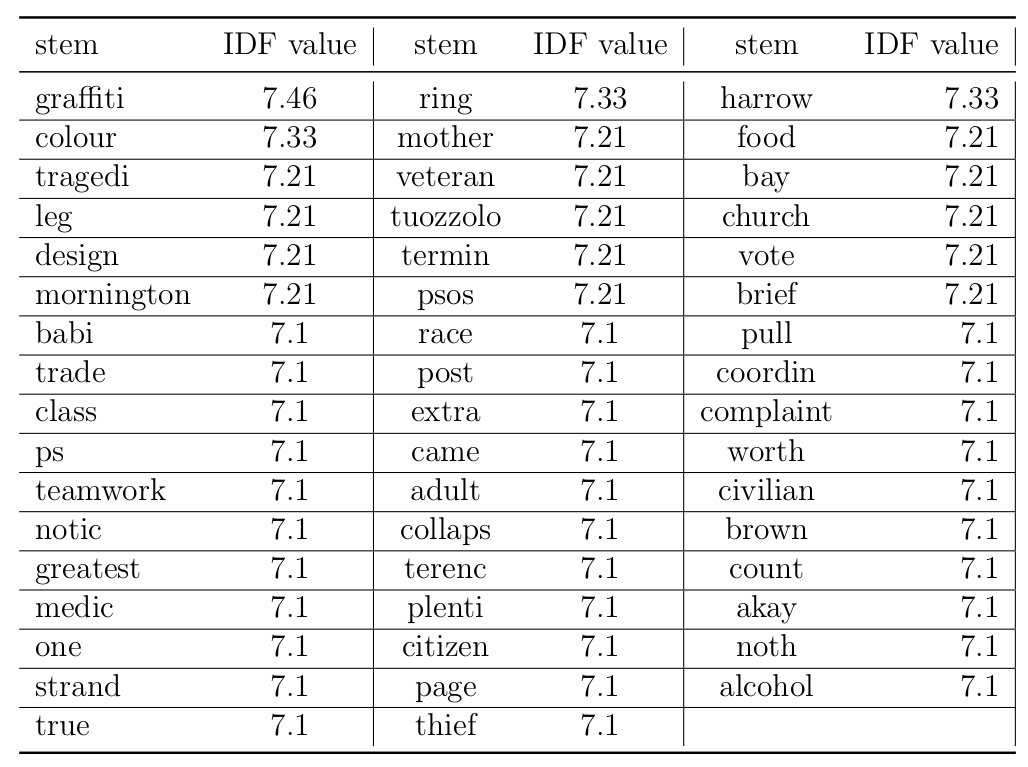
\includegraphics[scale=0.225]{images/idf_values.png}
        \caption{Top 50 IDF values}
        \label{fig:idf_values}
    \end{figure}
\end{frame}

\begin{frame}{TF-IDF vector}
    Once the IDF values for the terms have been calculated, the TF-IDF algorithm can be used to convert the text into a vector by multiplying the TF of the term with its IDF value as shown in Equation \ref{eq:tf_idf_equation}.

    The vector $v$ obtained is then normalized using the $L^2$ norm as follows,
    \begin{equation}
        v_{norm} = \frac{v}{\lVert v \rVert}
    \end{equation}
\end{frame}

\begin{frame}{Classification models}
    \begin{enumerate}
        \item Logistic Regression
        \item Support Vector Machine
        \item Random Forests
        \item Neural Network
    \end{enumerate}
\end{frame}

\begin{frame}{Logistic Regression}
    \begin{itemize}
        \item Regularized logistic regression
        \item Hypothesis function
        \begin{equation}
            \label{eq:regularized_logistic_regression}
            h_{\theta}(x) = \frac{1}{1 + {e}^{-{\theta}^{t}. x}}
        \end{equation}
    \end{itemize}
\end{frame}

\begin{frame}{Support Vector Machine}
    \begin{itemize}
        \item Soft margin
        \item RBF kernel
        \begin{equation}
            \label{eq:rbf_kernel}
            K(x, x^{'}) = exp(- \frac{{\lVert x - x^{'} \rVert}^{2}}{2 \sigma^{2}})
        \end{equation}
    \end{itemize}
\end{frame}

\begin{frame}{Random Forests}
    \begin{itemize}
        \item Criterion: gini
        \item Minimum sample split: 2
        \item Minimum sample leaf: 1
    \end{itemize}
\end{frame}

\begin{frame}{Neural network}
    \begin{itemize}
        \item Three layer network
        \item Activation function: ReLu
    \end{itemize}
\end{frame}

\begin{frame}{Training and testing}
    Dataset is seperated into training set and testing set using a 80/20 split.
\end{frame}

\begin{frame}{Training and testing}
    \begin{figure}[h]
        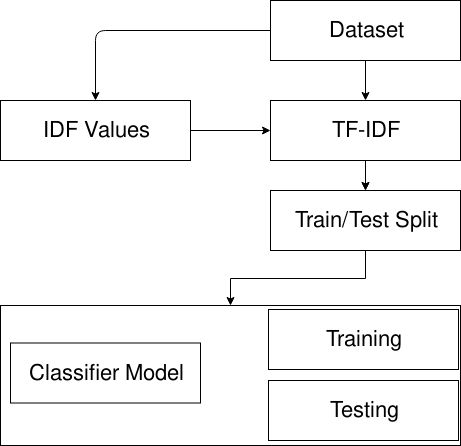
\includegraphics[scale=0.4]{images/training.png}
        \caption{Flow diagram for training and testing}
        \label{fig:training_testing}
    \end{figure}
\end{frame}

\begin{frame}{Prediction}
    \begin{figure}[h]
        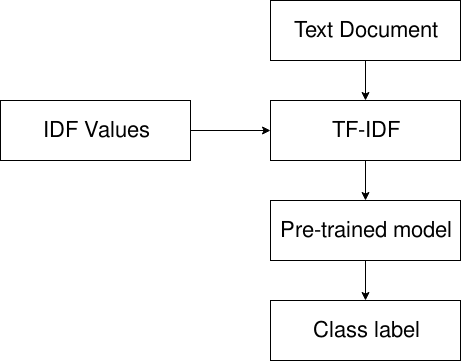
\includegraphics[scale=0.4]{images/prediction.png}
        \caption{Flow diagram for prediction}
        \label{fig:prediction}
    \end{figure}
\end{frame}
\section{Results}

\begin{frame}{Dataset visualization}
\begin{figure}[h]
    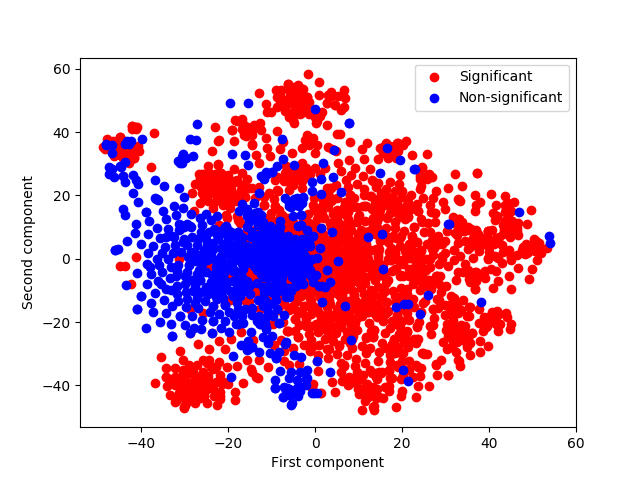
\includegraphics[scale=0.5]{images/data_visualization.png}
    \caption{Dataset visualization using t-SNE}
    \label{fig:dataset}
\end{figure}
\end{frame}

\begin{frame}{Test performance}
\begin{figure}[h]
    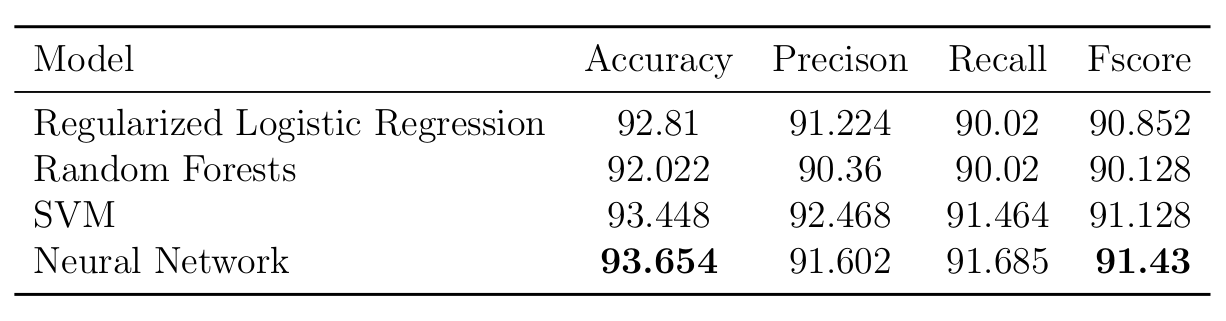
\includegraphics[width=\textwidth]{images/avg_performance.png}
    \caption{Average performance of classifiers on significant news dataset}
    \label{tbl:average_performance}
\end{figure}
\end{frame}

\section{Conclusion}

\begin{frame}{Summary}
\end{frame}

{\setbeamercolor{palette primary}{fg=black, bg=yellow}
\begin{frame}[standout]
  Questions?
\end{frame}
}

\appendix

\begin{frame}[allowframebreaks]{References}
    \bibliography{references}
    \bibliographystyle{unsrt}
\end{frame}

\end{document}
